\chapter{Basic Scrubbing}
At home you can take your time picking a lock, but in the field, speed is always essential.
This chapter presents a lock picking technique called \textit{scrubbing} that can quickly open most locks.

The slow step in basic picking (chapter 4) is locating the pin which is binding the most.
The force diagram (Figure 5.5) developed in chapter 5 suggests a fast way to select the correct pin to lift.
Assume that all the pins could be characterized by the same force diagram.
That is, assume that they all bind at once and that they all encounter the same friction.
Now consider the effect of running the pick over all the pins with a pressure that is great enough to overcome the spring and friction forces but not great enough to overcome the collision force of the key pin hitting the hull.
Any pressure that is above the at portion of the force graph and below the top of the peak will work.
As the pick passes over a pin, the pin will rise until it hits the hull, but it will not enter the hull.
See Figure 5.3.
The collision force at the sheer line resists the pressure of the pick, so the pick rides over the pin without pressing it into the hull.
If the proper torque is being applied, the plug will rotate slightly.
As the pick leaves the pin, the key pin will fall back to its initial position, but the driver pin will catch on the edge of the plug and stay above the sheer line.
See Figure 6.1.
In theory one stroke of the pick over the pins will cause the lock to open.

In practice, at most one or two pins will set during a single stroke of the pick, so several strokes are necessary.
Basically, you use the pick to scrub back and forth over the pins while you adjust the amount of torque on the plug.
The exercises in chapter 8 will teach you how to choose the correct torque and pressure.

You will find that the pins of a lock tend to set in a particular order. Many factors effect
this order (see chapter 9), but the primary cause is a misalignment between the center axis
of the plug and the axis on which the holes were drilled. See Figure 6.2. If the axis of the
pin holes is skewed from the center line of the plug, then the pins will set from back to front
if the plug is turned one way, and from front to back if the plug is turned the other way.
Many locks have this defect.

Scrubbing is fast because you don't need to pay attention to individual pins. You only
need to find the correct torque and pressure. Figure 6.1 summarizes the steps of picking a
lock by scrubbing. The exercises will teach you how to recognize when a pin is set and how
to apply the correct forces. If a lock doesn't open quickly, then it probably has one of the
characteristics described in chapter 9 and you will have to concentrate on individual pins.

\begin{table}
    \begin{enumerate}
        \item Insert the pick and torque wrench. Without applying any torque pull the pick out to
        get a feel for the stiffness of the lock's springs.
        \item Apply a light torque. Insert the pick without touching the pins. As you pull the
        pick out, apply pressure to the pins. The pressure should be slightly larger than the
        minimum necessary to overcome the spring force.
        \item Gradually increase the torque with each stroke of the pick until pins begin to set.
        \item Keeping the torque fixed, scrub back and forth over the pins that have not set. If
        additional pins do not set, release the torque and start over with the torque found in
        the last step.
        \item Once the majority of the pins have been set, increase the torque and scrub the pins
        with a slightly larger pressure. This will set any pins which have set low due to beveled
        edges, etc.
    \end{enumerate}
    \caption{Basic scrubbing.}
\end{table}

\begin{figure}
    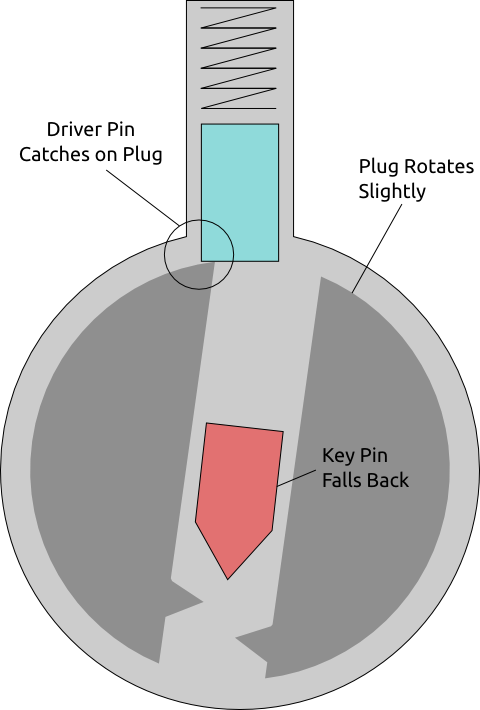
\includegraphics[scale=0.5]{figure6.1}
    \caption{Driver pin catches on plug}
\end{figure}

\begin{figure}
    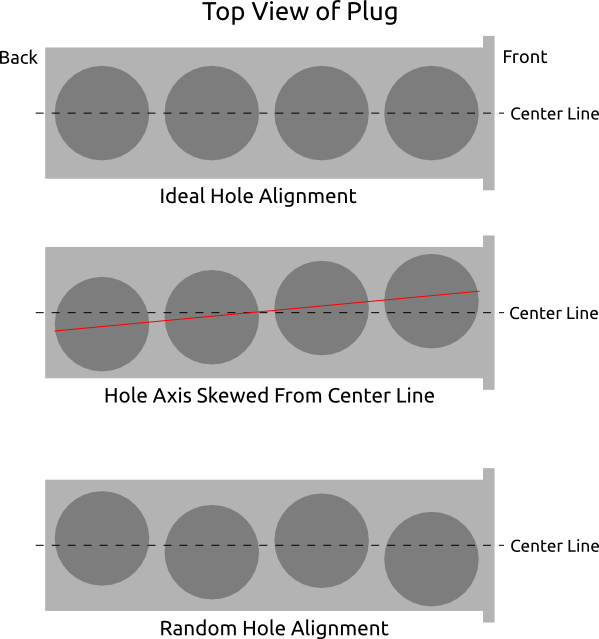
\includegraphics[width=\textwidth]{figure6.2}
    \caption{Alignment of plug holes}
\end{figure}
